\section{Concave Piecewise Likelihoods}
\label{sec:piecewise}

The linear algebraic solution to recover parameters for each clique
  $\sC$ presented in the previous section is easy to understand and
  analyze, but sensitive to noise. 
In this section we propose an alternate solution, optimizing the piecewise
  likelihoods, that is more robust to noise.
We show that under the same conditions for \algorithmref{directed}, the
  piecewise likelihoods are strictly concave, guaranteeing that
  gradient-based optimization will converge to the unique global
  optimum.

Consider a clique $\sC = \{h_{i_1}, \cdots h_{i_m}\} \in \sG$, with
  exclusive views $\sV = \{x_{v_1}, \cdots, x_{v_m}\}$. 
The piecewise likelihood of $\Sx{\sV}$ is,
\begin{align*}
  \sL_p(\Sx{\sV}) 
   &= \sum_{x \in \sD} \log \Pr( \Sx \sV ) \\
   &= \sum_{x \in \sD} \log \sum_{\Sh \sC} \Pr( \Sx \sV \given \Sh \sC ) \\
   &= \sum_{x \in \sD} \log \mH_\sC(\mOpp{v_{v_1}}{h_{i_1}}_{x_{v_1}}, \cdots, \mOpp{v_{v_m}}{h_{i_m}}_{x_{v_m}}) \\
   &= \sum_{x \in \sD} \log \mH_\sC \cdot \mOpp{\sV}{\sC}_x.
\end{align*}

The likelihood is concave in $\mH_\sC$; next, we show that it is
strictly concave, which guarantees a unique maximizer.
  
Taking the first derivative,
\begin{align}
  \grad_{\mH_\sC} \sL_p(\sX_\sV) 
  &= \sum_{x \in \sD} \frac{\mOpp{\sV}{\sC}_x}{\mH_\sC \cdot \mOpp{\sV}{\sC}_x} \nonumber \\ 
  &= \mOpp{\sV}{\sC}_x \diag(\tilde \mO_{\sV})^{-1} \mO_{\sV}, \label{eqn:lhood-grad}
\end{align}
  where $\tilde \mO_\sV$ is marginal distribution with parameters $\mH_\sC$.

Taking the second derivative.
\begin{align}
  \grad^2_{\mH_\sC} \sL_p(\Sx \sV) 
  &= \sum_{x \in \sD} \frac{\mOpp{\sV}{\sC}_x \mOpp{\sV}{\sC}_x^T}{(\mH_\sC \cdot \mOpp{\sV}{\sC}_x)^2} \nonumber \\
  &= \sum_{x \in \sD}\mOpp{\sV}{\sC}_x \mOpp{\sV}{\sC}_x^T \frac{(\mO_{\sV})_x}{(\tilde \mO_{\sV})^2_x} \nonumber \\
  &= \mOpp{\sV}{\sC} \diag(\mO_{\sV}) \diag(\tilde \mO_{\sV})^{-2} \mOpp{\sV}{\sC}^T. \label{eqn:lhood-hess}%
\end{align}

As $\tilde \mO_\sV, \tilde \mO_\sV \succ 0$ and $\mOpp{\sV}{\sC}$ are
full rank and stochastic, $\grad^2_{\mH_\sC} \sL_p(\Sx \sV) \succ 0$.

\algorithmref{piecewise} reviews our algorithm.

\begin{algorithm}
  \caption{\LearnPiecewise}
  \label{algo:piecewise}
  \begin{algorithmic}
    \REQUIRE A graphical model $\sG$ satisfying \textbf{(P1)}, \textbf{(P2)}, data $\sD$
    \ENSURE Parameters $\theta$ for $\sG$

      \FOR{$h \in H$} 
        \STATE Apply \TensorFactorize for each bottleneck $h$ and learn parameters $\Pr(x \mid h) ~ \forall x \in \sB(h)$.

%    \COMMENT{Recover observation potentials $O$ using bottlenecks}
      \ENDFOR
%      \COMMENT{\textbf{Step 2:} Recover clique potentials from the piecewise likelihood.}
      \FOR{every clique $\sC = \{h_1, \cdots, h_m\} \in \sG$} 
      \STATE Let $x_\sC = \{x_1, \cdots, x_m\}$.
      \STATE $\hat \mH_\sC = \arg\max_{\mH_\sC \in \Delta_{k^m-1}} \E_{\vec x_\sC}[ \log \mH_\sC( \pinv O_{x_1}, \cdots, \pinv O_{x_m} ) ]$.
%      Run expectation-maximization to convergence on the piecewise likelihood \eqref{eqn:piecewise}, over data $\{\vec x_\sC : x \in \sD\}$
      \ENDFOR
  \end{algorithmic}
\end{algorithm}

\subsection{Comparison with Method of Moments}

By Cramer-Rao, we know that the asymptotic variance of the
  maximum-likelihood estimator is the best we can do.
We'll now show that the asymptotic variance of the method of moments is strictly worse.

\begin{lemma}(Asymptotic variance for the likelihood)
  \label{lem:pw-variance}
  The asymptotic variance in the recovered parameters $Z_{\sC}$ by optimizing the likelihood is,
  \begin{align*}
    \sqrt{n}(\hat Z_{\sC} - Z_{\sC}^*) \convind \sN( 0, \pinvt{\mOpp{\sV}{\sC}} \Sigma_\sV \pinv{\mOpp{\sV}{\sC}} ),
  \end{align*}
  where $\Sigma_\sV$ is the variance of the moment estimates, 
  \begin{align*}
    \Sigma_\sV &= \diag(M_\sV) - M_\sV M_\sV^T.
  \end{align*}
\end{lemma}
\begin{proof}
  By the delta-method, 
  \begin{align*}
    \sqrt{n}(\hat Z_{\sC} - Z_{\sC}) \convind \sN( 0, \grad^2 \sL_p(\vec x_\sC)^{-1} \Var \grad \sL_p(\vec x_\sC)\grad^2 \sL_p(\vec x_\sC)^{-1}).
  \end{align*}

  From \equationref{lhood-grad}, we get
  \begin{align*}
    \Var \grad \sL_p(\vec x_\sC) &= \mOpp{\sV}{\sC} \diag(\tilde M_\sV) \Sigma_\sV \diag(\tilde M_\sV) \mOpp{\sV}{\sC}^T .
  \end{align*}

  Finally, using \equationref{lhood-hess}, we have
  \begin{align*}
    \Sigma_{Z_\sC} 
      &= \grad^2 \sL_p(\vec x_\sC)^{-1} \Var \grad \sL_p(\vec x_\sC)\grad^2 \sL_p(\vec x_\sC)^{-1}) \\
      &= \pinvt{\mOpp{\sV}{\sC}} \diag(\tilde M_\sV) \Sigma_\sV \diag(\tilde M_\sV) \pinv{\mOpp{\sV}{\sC}}.
  \end{align*}
\end{proof}

\begin{corollary}
  The asymptotic variance of optimizing the log-likelihood, $\Sigma_p$
  is strictly less than that of the moment-matching objective
  $\Sigma_m$; $\Sigma_p \succ \Sigma_m \succ 0$.
\end{corollary}
\begin{proof}
  From \lemmaref{mom-complexity}, we have the asymptotic variance of the method of moments estimator, $\hat Z_\sC^(m)$ is,
  \begin{align*}
    \sqrt{n}(\hat Z_\sC - Z_\sC) \convind \sN(0, \pinvt{\mOpp{\sV}{\sC}} \Sigma_\sV \pinv{\mOpp{\sV}{\sC}}).
  \end{align*}

  From the previous lemma, we have the asymptotic variance of the piecewise likelihood estimator, $\hat Z_\sC^(p)$ is,
  \begin{align*}
    \sqrt{n}(\hat Z_{\sC} - Z_{\sC}) \convind \sN( 0, \pinvt{\mOpp{\sV}{\sC}} \diag(\tilde M_\sV) \Sigma_\sV \diag(\tilde M_\sV) \pinv{\mOpp{\sV}{\sC}} ).
  \end{align*}

  Note that $\Sigma_p = \diag(\tilde M_\sV) \Sigma_m \diag(\tilde M_\sV)$; as $M_\sV$ is stochastic, $\Sigma_m \succ \Sigma_p \succ 0$. 
\end{proof}

We know that $\|\hat Z_c - Z_c\|^2_2 = O(\Tr(\Sigma))$; with this
analysis, the piecewise estimator requires $\Tr(\diag(M_\sV) \Sigma_m
\diag(M_\sV))$ samples, which is $\approx \frac{1}{d} \Tr(\Sigma_m)$;
i.e. you require a factor of $d$ less.

\paragraph{Intuition}

Consider a hidden Markov model \figureref{fig:examples-hmm} with
  2 states ($k=2$), but an arbitrary number of emissions, $d$. 
After learning the observation potentials $O$ in step 1 of
  \algorithmref{piecewise}, the log-likelihood objective for $\pi$ is,
\begin{align}
  \sL_p(x_1) &= \sum_{x_1} \log( \pi_1 O_{1,x_1} + (1-\pi_1) O_{2,x_1} ).
\end{align}

Empirically, we observe that optimizing the piecewise objective gives
  better solutions with finite samples.

\begin{figure}
  \centering
  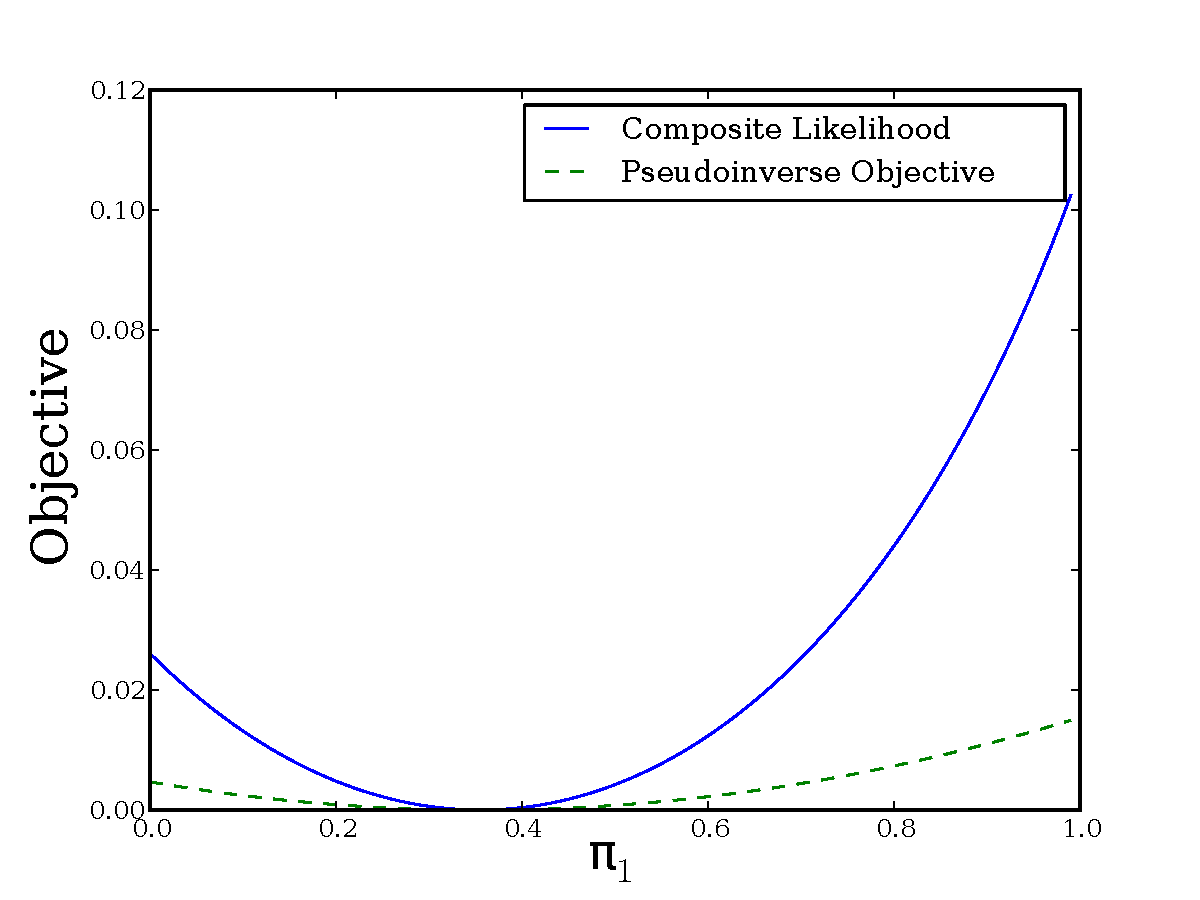
\includegraphics[width=\columnwidth]{figures/piecewise-objective.pdf}
  \caption{Comparing the piecewise objective with the moment-matching objective for just one parameter}
  \label{fig:piecewise-objective}
\end{figure}

The negative log-likelihood is more concave than the moment-reconstruction loss (\figureref{piecewise-objective})

\subsection{More examples}

We will now instantiate our algorithm for several examples, illustrated in \figureref{examples}.

\begin{figure}
  \subfigure[Hidden Markov Model] {
    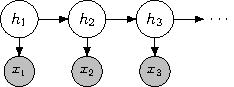
\includegraphics{figures/hmm.pdf}
    \label{fig:examples-hmm}
  }
%  \subfigure[Directed grid model] {
%    \label{fig:examples-grid}
%    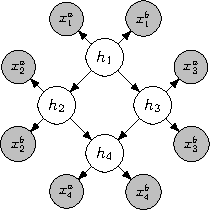
\includegraphics{figures/grid.pdf}
%  }
  \subfigure[Tree model] {
    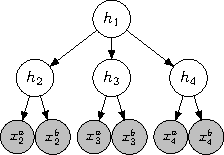
\includegraphics{figures/tree.pdf}
    \label{fig:examples-tree}
  }
  \caption{Examples of models in the bottleneck family\define.}
  \label{fig:examples}
\end{figure}

\paragraph{Hidden Markov Model}

In this example (\figureref{fig:examples-hmm}), we assume that
  $\Pr(x_i|h_i) = O  ~\forall i$  and that $\Pr(h_{i+1} | h_i)
  = T ~\forall i$ (i.e. we have parameter sharing).
Note that while the first (and last) hidden variables $h_1, h_T$ in the
  sequence are not bottlenecks, they still have exclusive views ($x_1$ and
  $x_T$ respectively) whose parameters we know because they share
  parameters, $O$.
In step 1 of our algorithm, we use the bottleneck $h_2$ with views $x_1,
  x_2, x_3$ and solve $O$.
In step 2 of our algorithm, we can recover $\pi$ by solving for the
  unary clique $\{h_1\}$ and recover $T$ from the clique $\{h_{1},
  h_{2}\}$.

As a further point, because we have so much parameter sharing, we can
  aggregate over all triples when estimating $O$ and over pairs when
  estimating $T$.

\paragraph{Latent Tree Structure}

In the latent tree structure (\figureref{fig:examples-tree}), let the
  parameters be $\Pr(h_i) = \pi$, $\Pr(h_i | h_1) = T ~i \in \{2,3,4\}$
  and $\Pr(x^a_i | h_i) = \Pr(x^b_i | h_i) = O ~i \in \{2,3,4\}$.
Note that while $h_1$ is not directly connected to an observed variable,
  it is still a bottleneck, with views $x^a_2, x^a_3, x^a_4$.

In step 1, we recover the parameters $O$ from the bottleneck $h_2$ with
  views $\{x^a_2, x^b_2, x^a_3\}$. We also recover the conditional moments
  $\mOpp{2}{1}$, $\mOpp{3}{1}$, $\mOpp{4}{1}$ for $h_1$. 
In step 2, we can recover $\pi$ from the clique $\{h_1\}$, using any
  one of views (they are all exclusive). 
To recover $T$ from the clique $\{h_1, h_2\}$, we use the views $x^a_2$
  (exclusive to $h_2$) and $x^a_3$ (exclusive to $h_3$). Note that while
  $x^a_3$ is also a view for $h_2$, $x^a_3$ is independent of $h_2$ given
  $h_1$.


\paragraph{Aggregating observations}
\todo{This section}
When we have multiple observed variables for a hidden variable, it is
  always beneficial to aggregate over them.
Note that $O_h$ will have rank atleast that of $O$; this encodes the
  intuitive fact that we might be able to identify $h$ from multiple
  observed variables even if we can not identify it from a single
  observed variable. 
Suppose $x_\sB(h) = \{x_1, x_2, \cdots, x_l\}$, let $O_h \in
  \Re^{D^l \times K}$ be an
  aggregated observation potential, such that $O_h(x_1, x_2, \cdots,
  x_l) = \mH(x_1|h) \mH(x_2|h) \cdots \mH(x_l|h)$.
Given \assumptionref{full-rank}, $O_h$ have rank $K$.
After step 1, $O_h$ is a known quantity.

